\chapter{Resultados y discusión}

La composición de imágenes satelitales de radiancia en la Ciudad de México (Figura~\ref{radiancetrends}) muestra cualitativamente que los niveles más altos de radiancia promedio se encuentran en la fracción norte-centro de la ciudad, lo que naturalmente, coincide con la mancha urbana. Dada esta distribución, se considera que un observador está <<dentro de la ciudad>> cuando se encuentra en alguno de los Sectores Urbanos mostrados en el Mapa CL-CDMX y <<fuera de la ciudad>> cuando está fuera de ellos, lo que corresponde con suelo de conservación. 

\section{Tendencias de radiancia promedio en las alcaldías de la Ciudad de México}

Por efectos de representatividad se selecionaron las siguientes figuras elaboradas con el software \textit{Radiance Light Trends} que muestran las tendencias de radiancia promedio en la alcaldía Gustavo A. Madero (GAM, densamente poblada), Milpa Alta (MA, menos poblada, con mayoría de territorio en suelo de conservación) y en el polígono de Ciudad Universitaria que contiene la REPSA (CU). El resto de las tendencias por alcaldía se encuentran en el \textbf{\autoref{chap:anexos}}.

\begin{figure}[htb]
  \centering
    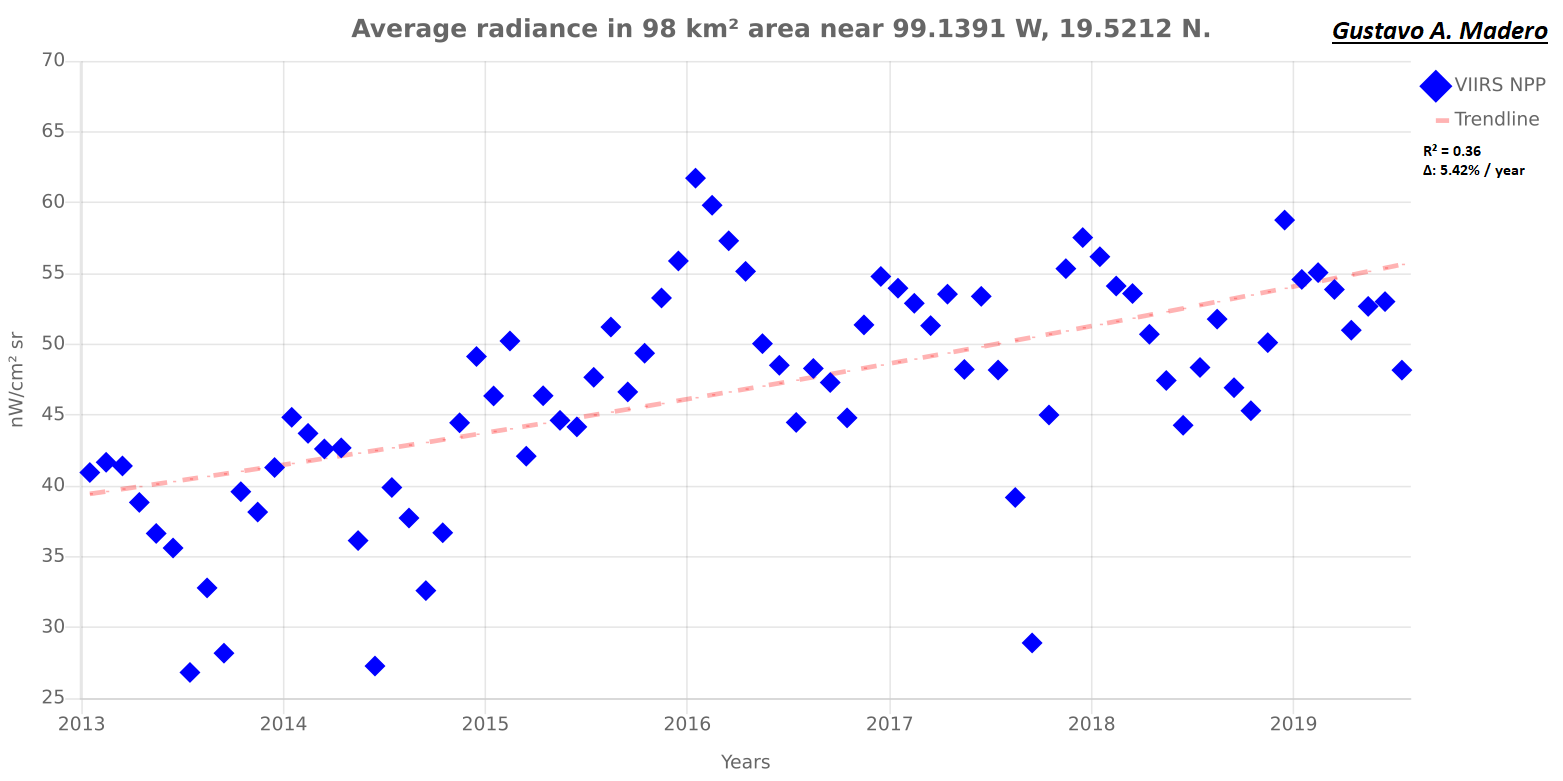
\includegraphics[width=1\textwidth]{GAM}
  \caption{Tendencia de radiancia promedio para la alcaldía Gustavo A. Madero}
  \label{radiancetrendsgam}
\end{figure}

\newpage


\begin{figure}[H]
  \centering
    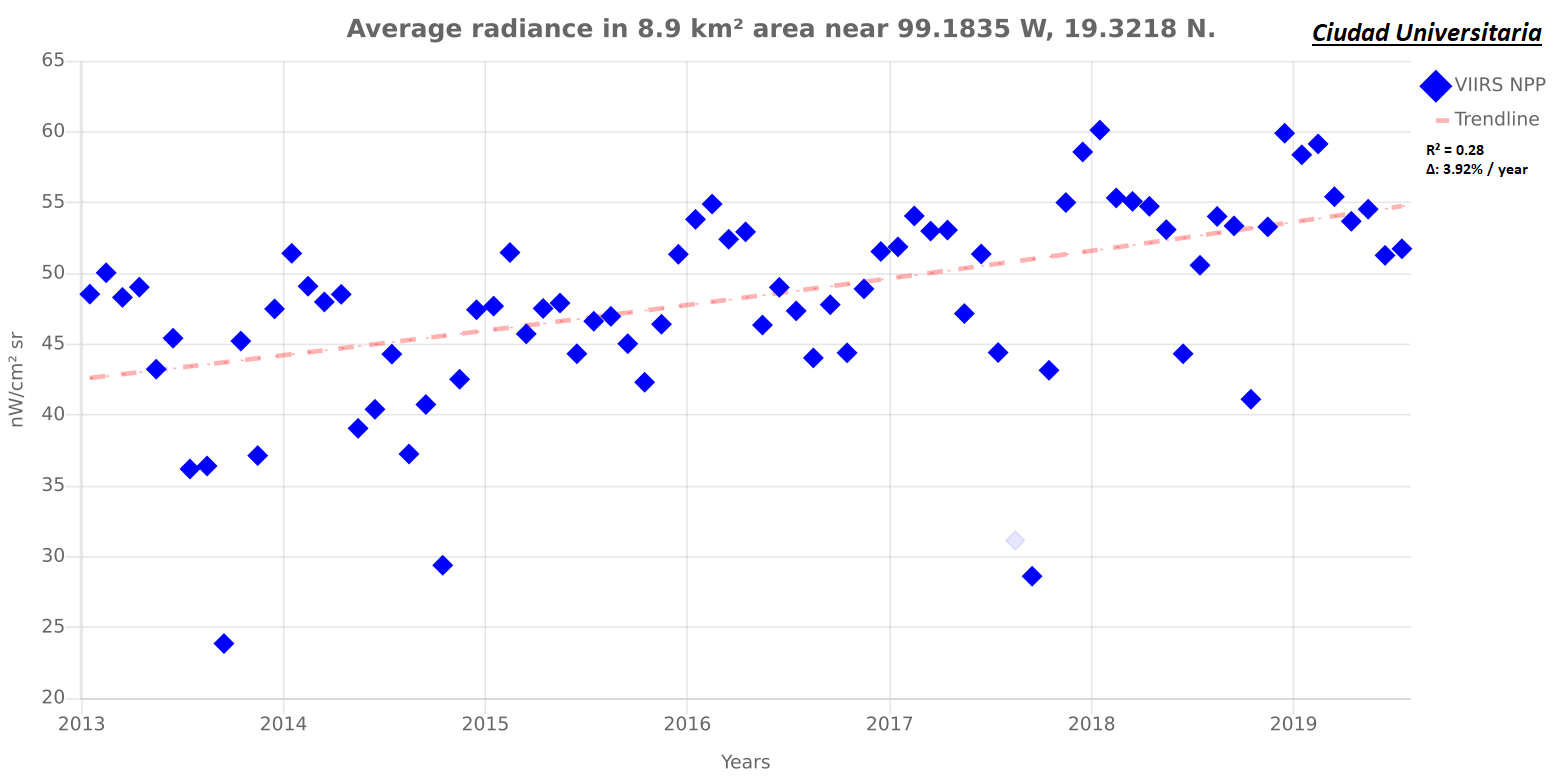
\includegraphics[width=1\textwidth]{CU}
  \caption{Tendencia de radiancia promedio para Ciudad Universitaria}
  \label{radiancetrendscu}
\vspace{20mm} 
    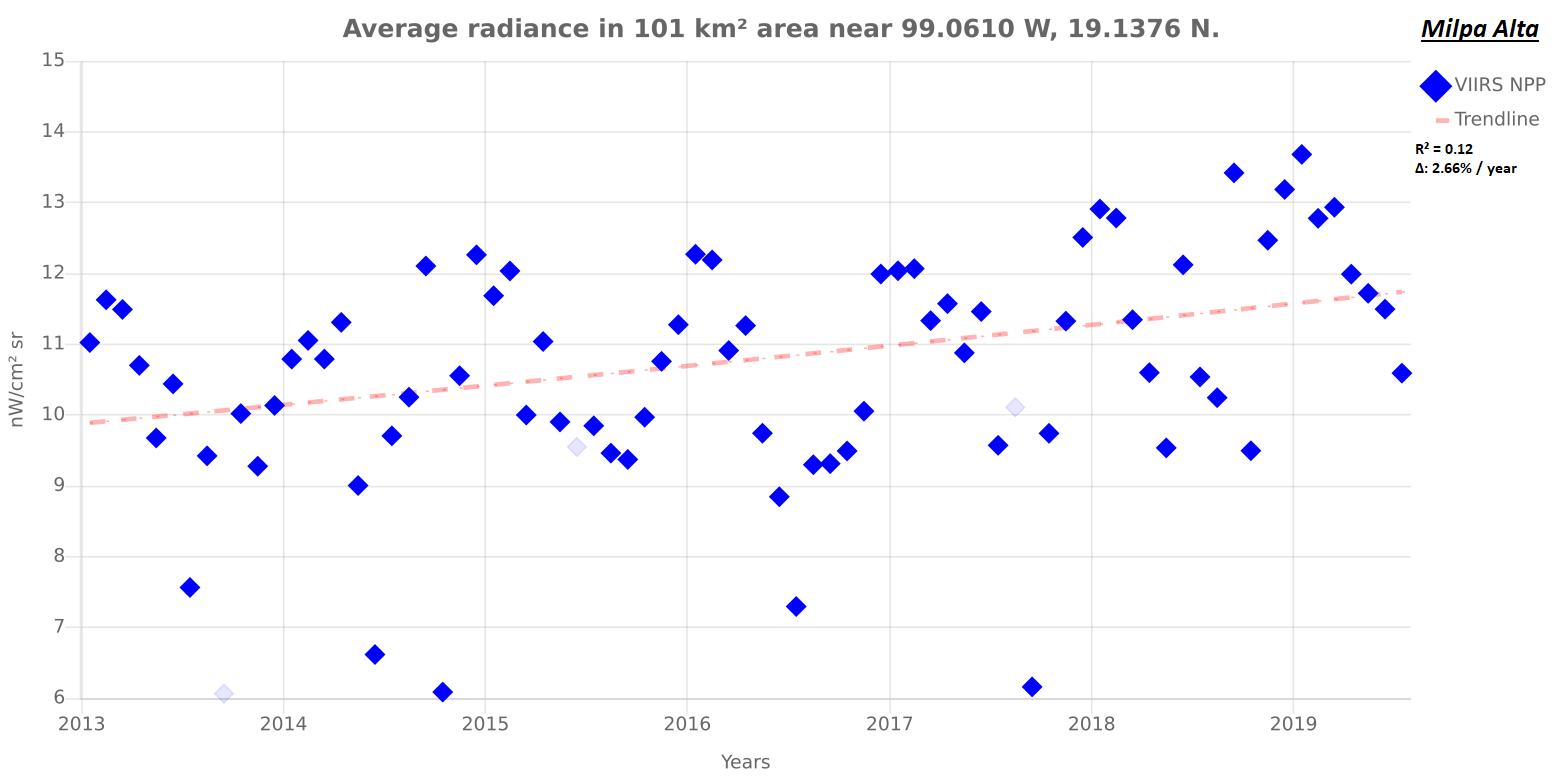
\includegraphics[width=1\textwidth]{MA}
  \caption{Tendencia de radiancia promedio para la alcaldía Ciudad Universitaria}
  \label{radiancetrendsma}
\end{figure}
\blindtext


\newpage

Como se muestra en el \textbf{Inventario de Alumbrado Público de la Ciudad de México}, hoy en día el principal tipo de fuente de luz del alumbrado público de la Ciudad de México es la lámpara de halogenuros metálicos. Sin embargo, de manera histórica, el número de luminarias y sus características han ido cambiando, lo que sumado a la fluctuación de  las luminarias residenciales y privadas ha tenido efecto en las tendencias de radiancia en las diferentes alcaldías de la ciudad.\\

De acuerdo con \cite{Universal2017} durante 2015 se destinaron 2600 millones de pesos mexicanos para el programa <<Iluminemos Tu Ciudad>>, que llevó a cabo el cambio de luminarias en vías primarias y secundarias de la Ciudad de México. Se menciona este hecho como la actualización de una <<tecnología de la década de 1990 por una más limpia>>.\\

La fuente de luz de las antiguas luminarias mencionadas era de halogenuros metálicos con un tubo de descarga de cuarzo mientras que las nuevas también tienen fuente de de halogenuros metálicos pero con la diferencia que el tubo de descarga es de cerámica, lo que algunos fabricantes mencionan 10-20\% más eficiente \citep{EMB2007}.\\

En pocas palabras, la dependencia espectral del alumbrado de la ciudad no cambió durante la aplicación del programa. En este punto es importante mencionar que la cualidad de <<limpia>> a la que los encargados del programa se refieren, no tiene nada que ver con CL sino con la diferencia en el consumo de las lámparas: mientras que las antiguas consumían 250 W, las nuevas consumen 140 W.\\ 

No obstante, durante el programa se instalaron 100 mil nuevas luminarias lo que en términos totales supone un ahorro de 27,000 kW h$^-1$ al día y 118,260 MW h$^-1$ al año; esto corresponde a menos del 1\% del consumo de energía eléctrica de la ciudad (véase la \textbf{\autoref{subsec:consumoenergiaelectrica}}). El resultado de este cálculo parece indicar que el programa no fue en realidad llevado a cabo pensando en iluminación <<más limpia>>, lo que se confirma con el conflicto de interés que lo caracterizó, en que el total de la inversión se asignó a empresas con antecedentes de incumplimiento pertenecientes a familiares del titular de Obras Públicas de la Ciudad de México de ese entonces \citep{Sinembargo2015}.\\ 

A pesar de todo, el programa <<Iluminemos Tu Ciudad>> hizo honor a su nombre y el VIIRS DNB logró captarlo desde el espacio: de 2015 a 2016 se observa un marcado aumento en los niveles de radiancia promedio en la mayoría de las alcaldías (Figura~\ref{radiancetrendsgam}, \textbf{\autoref{chap:anexos}}). Mientras tanto, otras delegaciones cuya mayoría de territorio se encuentra fuera de la ciudad no muestran un crecimiento exponencial en radiancia promedio (Figura~\ref{radiancetrendsma}) debido a que en esas zonas la población es extremadamente baja. Para el caso de Ciudad Universitaria (Figura~\ref{radiancetrendscu}) se observa también un crecimiento exponencial en radiancia promedio aunque a una velocidad más lenta con respecto a la mayoría de las alcaldías.\\ 


Referente a los valores promedio de radiancia se registran los más altos en alcaldías dentro de la ciudad con el valor más extremo (86 nW sr$^{-1}$  cm$^{-2}$) obtenido para la alcaldía Venustiano Carranza en 2016, lo que no resulta extraño cuando se remite al dato destacado por el \textit{City Manager} de la Ciudad de México acerca de que, en la zona de Los Arenales en la alcaldía Venustiano Carranza <<todo está encendido>> en comparación a otras zonas de la Ciudad de México \citep{Universal2017}.\\

\newpage

Por otro lado, valores promedio de radiancia muy bajos de hasta 6 nW sr$^{-1}$  cm$^{-2}$ se registraron para la alcaldía Milpa Alta, mientras que para Ciudad Universitaria, los valores se registran alrededor de los promedios observados en otras alcaldías dentro de la ciudad.\\

Por lo tanto, los valores de radiancia promedio medidos por el VIIRS DNB para la Ciudad de México están comprendidos entre 6 x 10$^{-5}$ y 8.5 x 10$^{-4}$ W sr$^{-1}$ m$^{-2}$, valores por encima del máximo natural registrado (10$^{-6}$ W sr$^{-1}$  m$^{-2}$), por lo que se puede hablar de la presencia de CL en todo el territorio de la Ciudad de México.\\ 

El futuro en cuestiones de CL no pinta bien al pensar en el panorama planteado por la Agencia de Gestión Urbana que sumándose a la tendencia global de las ciudades, pretende instalar <<dispositivos que iluminan mejor y son más eficientes como la tecnología LED>> en vías primarias de la ciudad \citep{Universal2017}. Véase la \textbf{\autoref{subsec:consecuenciascl}} en que se reporta el LED como la fuente de luz con mayor potencial en términos de CL.\\ 


\section{Gráficas tipo \textit{all sky} de distribución de radiancia}

En esta sección se enfoca el problema de la CL desde otra perspectiva diferente a las mediciones promedio satelitales, se lleva a cabo el análisis del brillo del cielo nocturno percibido por un observador en superficie de acuerdo con las salidas del modelo \textit{SkyGlow}.\\ 

Para tales análisis se seleccionaron los mismos casos particulares de la sección anterior: un observador dentro de la alcaldía Gustavo A. Madero (coordenadas: 19.47\grad, -99.14\grad), alcaldía Milpa Alta (coordenadas: 19.09\grad, -99.15\grad) y la Zona Núcleo Oriente de la REPSA dentro de Ciudad Universitaria (coordenadas: 19.31\grad, -99.18\grad).\\

\newpage

\begin{figure}[H]
  \centering
    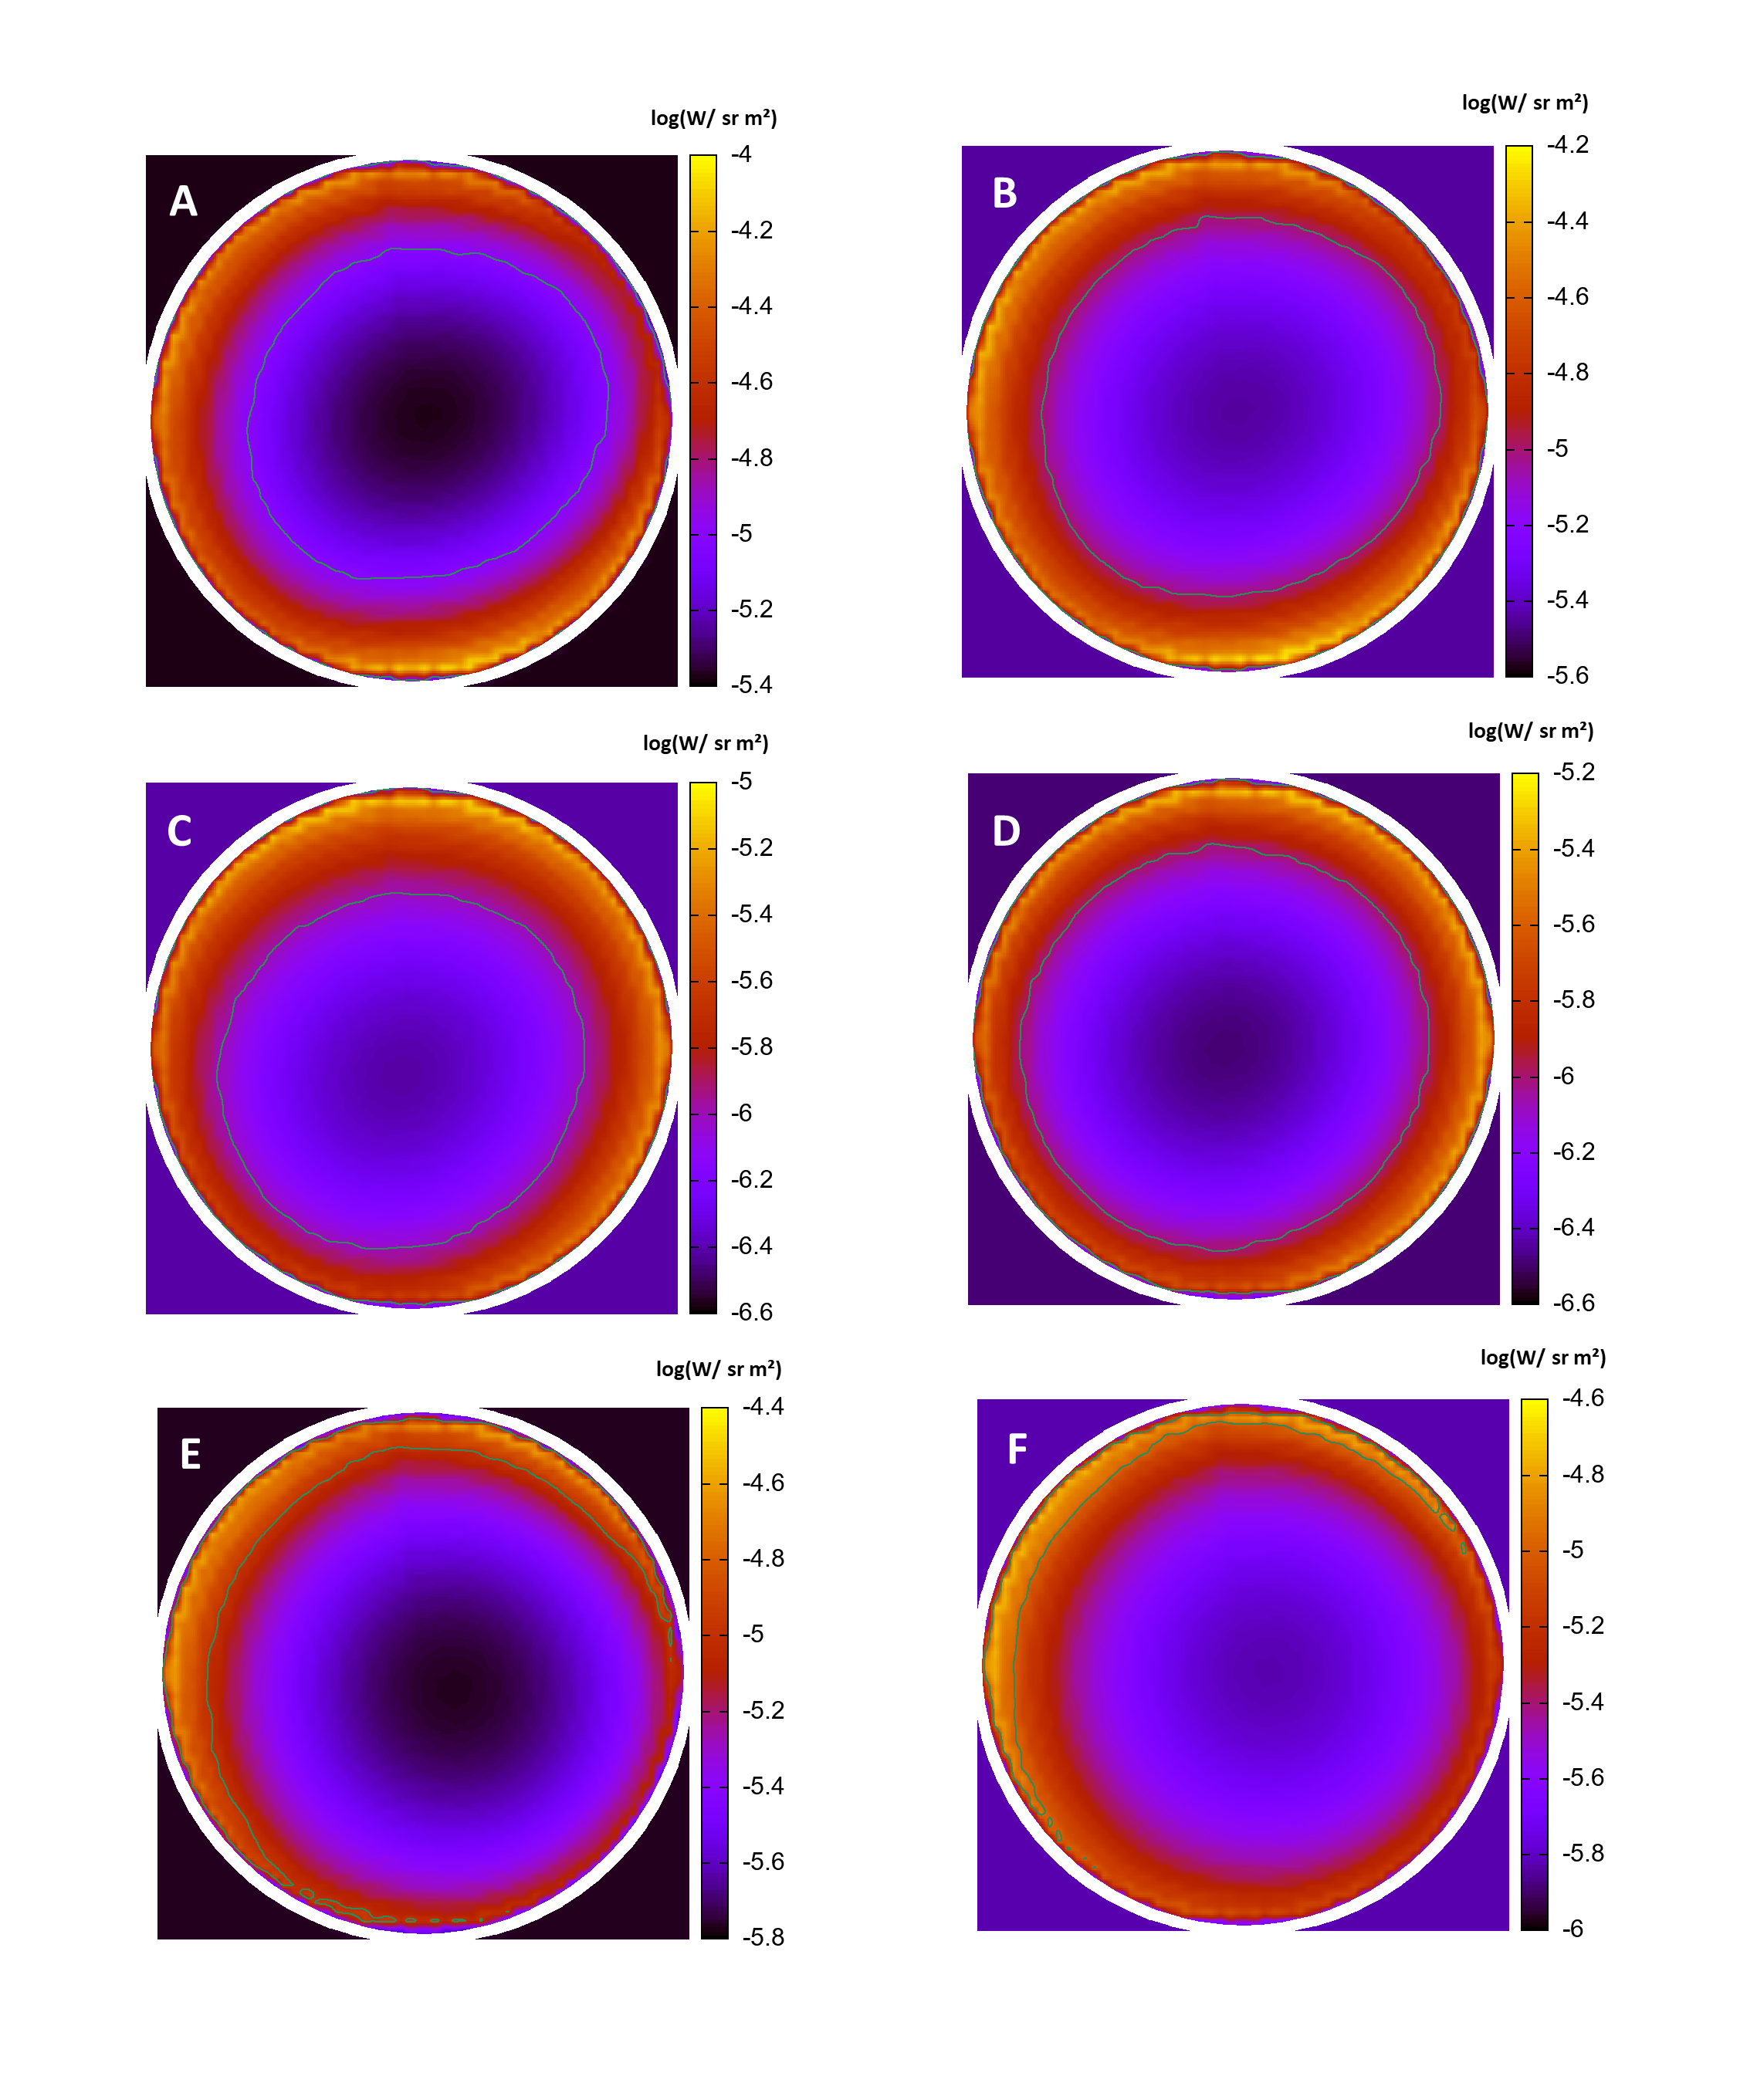
\includegraphics[width=1\textwidth]{1}
  \caption{Gráficas tipo \textit{all sky} para condiciones de cielo despejado con A) Fondo Promedio para GAM, B) Especies Carbonosas para GAM, C) Caso de A) para MA, D) Caso de B) para MA, E) Caso de A) para CU y F) Caso de B) para CU} 
  \label{1}
\end{figure}


\newpage

\section{Experimentos numéricos}

Por el potencial ahorro económico que supone, se está llevando a cabo una gran sustitución de instalaciones de alum-
brado público cambiando fuentes tradicionales -en muchos casos de vapor de sodio a alta presión- por LED.

\newpage

\subsection{Influencia del aerosol atmosférico en la distribución de radiancia}

\begin{figure}[H]
  \centering
    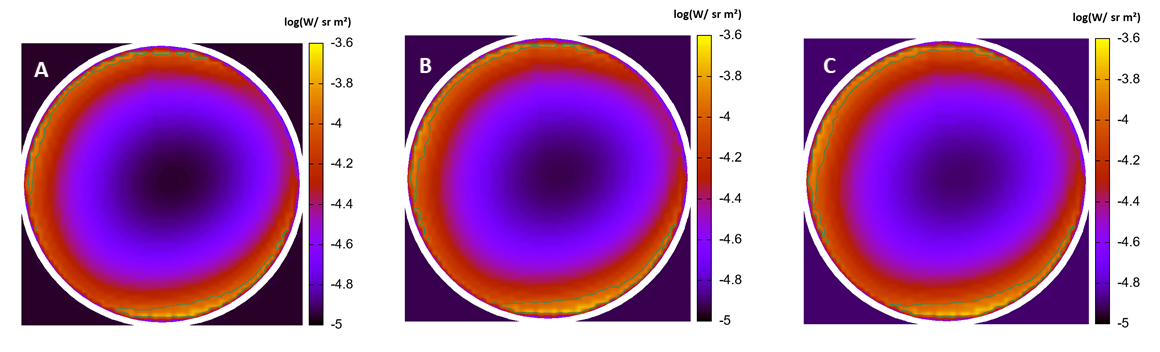
\includegraphics[width=1\textwidth]{2}
  \caption{Gráficas tipo \textit{all sky} para condiciones de cielo despejado para GAM en A) Invierno Seco, B) Primavera Seca y C) Temporada Lluviosa} 
  \label{2}
\end{figure}}

\begin{figure}[H]
  \centering
    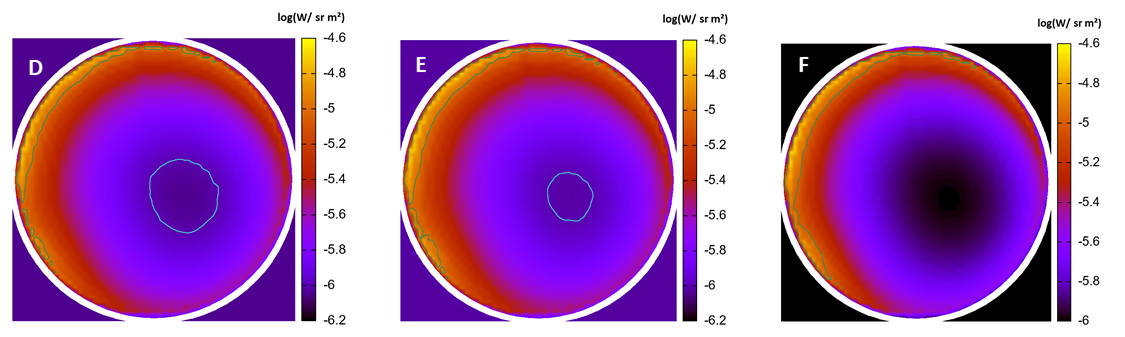
\includegraphics[width=1\textwidth]{3}
  \caption{Gráficas tipo \textit{all sky} para condiciones de cielo despejado para MA en A) Invierno Seco, B) Primavera Seca y C) Temporada Lluviosa} 
  \label{3}
\end{figure}

\begin{figure}[H]
  \centering
    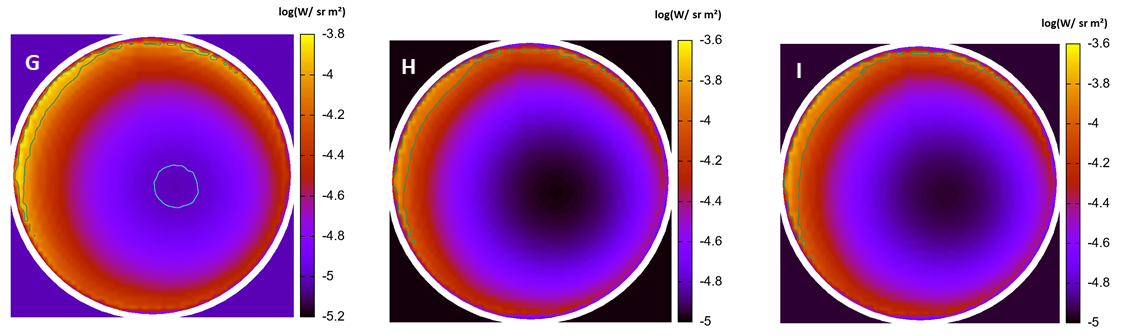
\includegraphics[width=1\textwidth]{4}
  \caption{Gráficas tipo \textit{all sky} para condiciones de cielo despejado para CU en A) Invierno Seco, B) Primavera Seca y C) Temporada Lluviosa} 
  \label{4}
\end{figure}

\newpage

\subsection{Influencia de la nubosidad en la distribución de radiancia}

\begin{figure}[H]
  \centering
    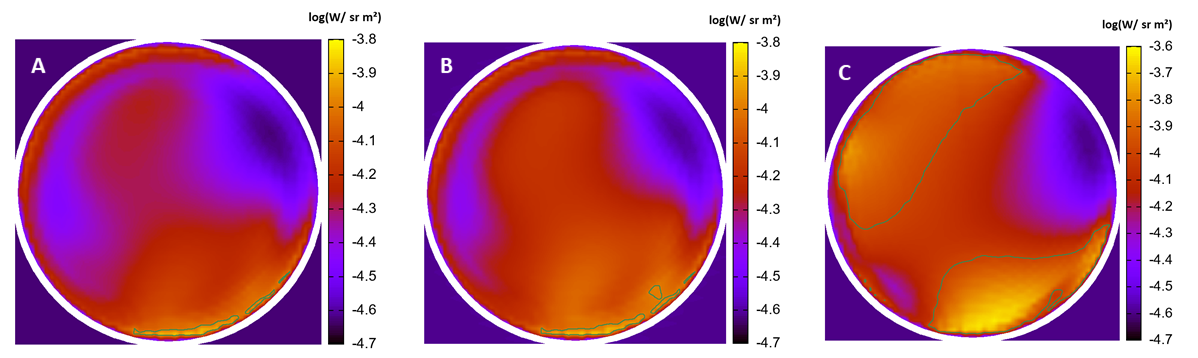
\includegraphics[width=1\textwidth]{5}
  \caption{Gráficas tipo \textit{all sky} para condiciones de cielo nublado para GAM con A) Nube altocumulus, B) Nube Altostratus y C) Nube stratus} 
  \label{5}
\end{figure}

\begin{figure}[H]
  \centering
    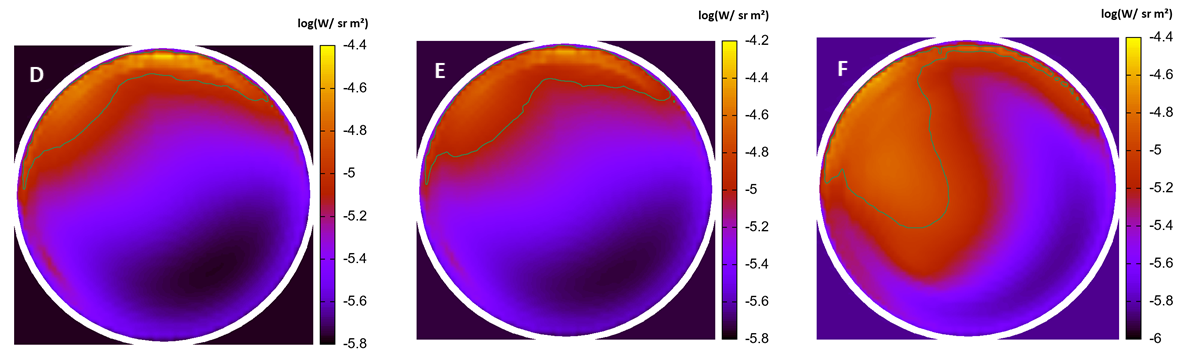
\includegraphics[width=1\textwidth]{6}
  \caption{Gráficas tipo \textit{all sky} para condiciones de cielo nublado para MA con A) Nube altocumulus, B) Nube Altostratus y C) Nube stratus} 
  \label{6}
\end{figure}

\begin{figure}[H]
  \centering
    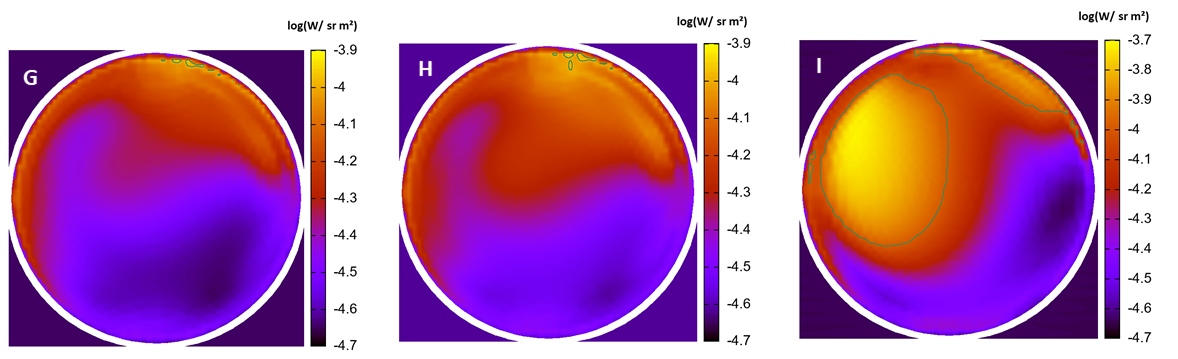
\includegraphics[width=1\textwidth]{7}
  \caption{Gráficas tipo \textit{all sky} para condiciones de cielo nublado para CU con A) Nube altocumulus, B) Nube Altostratus y C) Nube stratus} 
  \label{7}
\end{figure}

\newpage

\subsection{Cambio del tipo de luminarias en la Ciudad de México}

\begin{figure}[H]
  \centering
    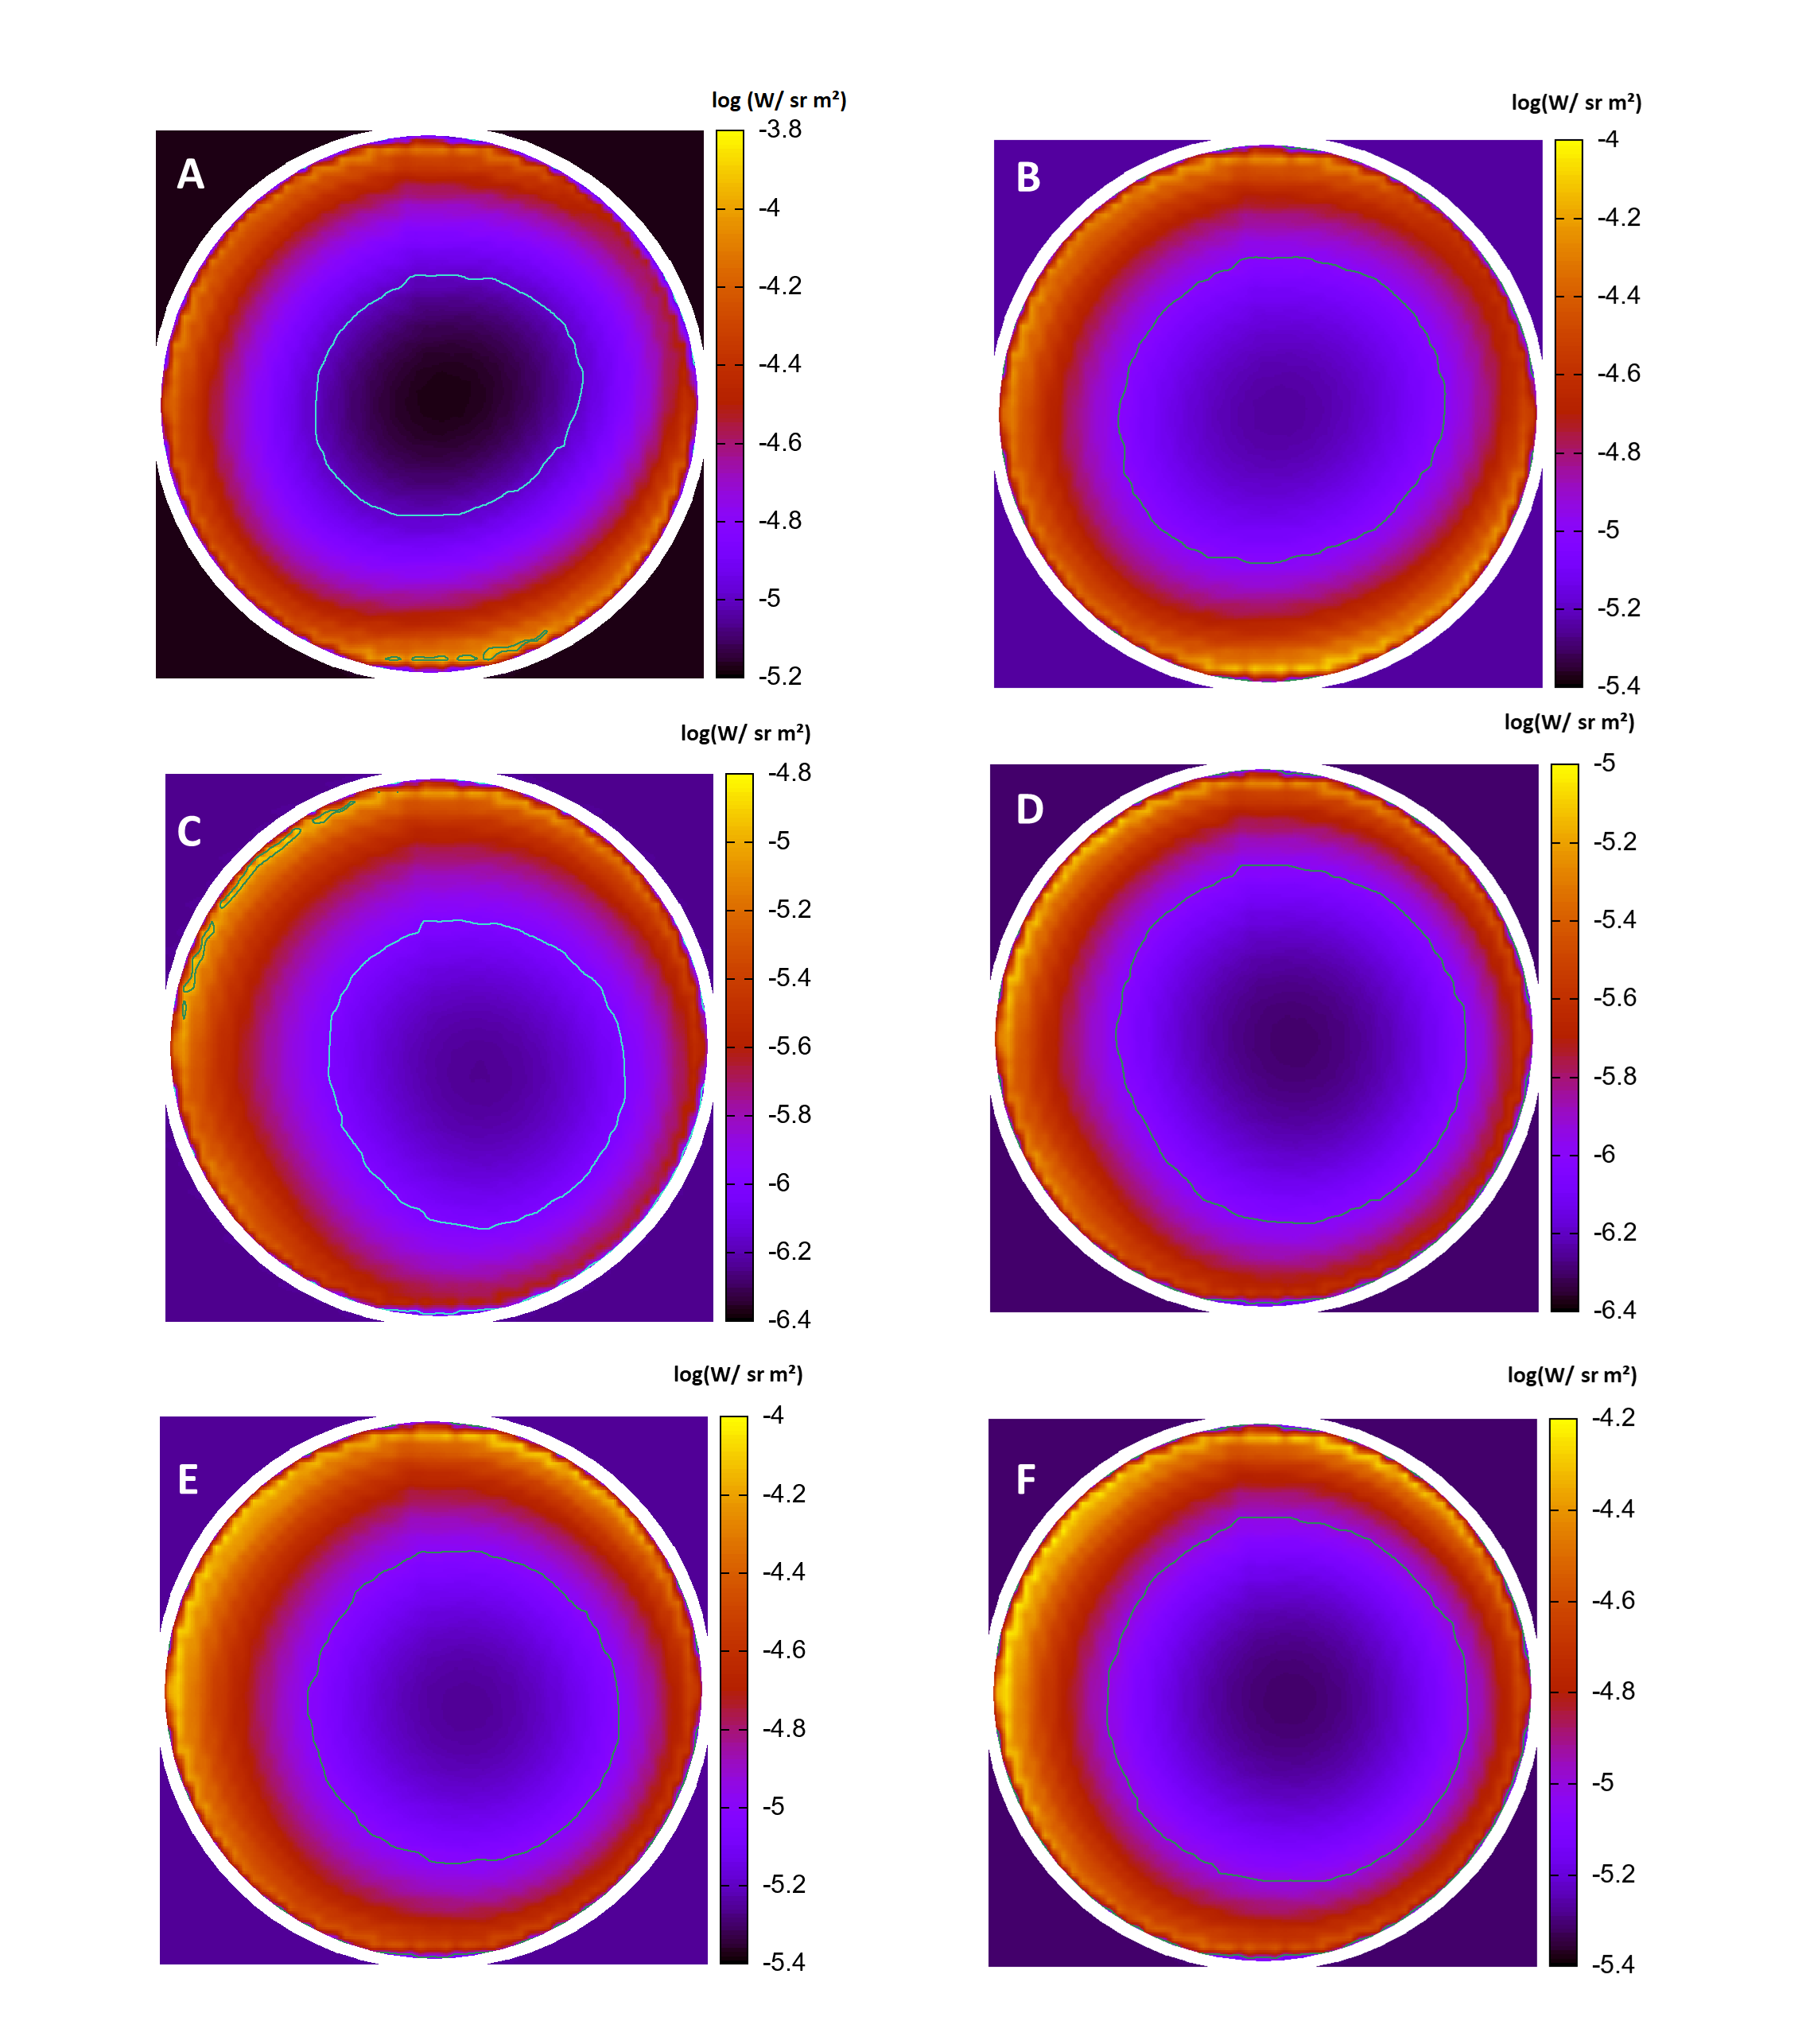
\includegraphics[width=1\textwidth]{8}
  \caption{Gráficas tipo \textit{all sky} para condiciones de cielo despejado con tipo de luminaria LED con A) Fondo Promedio para GAM, B) Especies Carbonosas para GAM, C) Caso de A) para MA, D) Caso de B) para MA, E) Caso de A) para CU y F) Caso de B) para CU} 
  \label{1}
\end{figure}

\newpage

\section{Mapa CL-CDMX}
\label{sec:mapacl}

\begin{figure}[H]
  \centering
    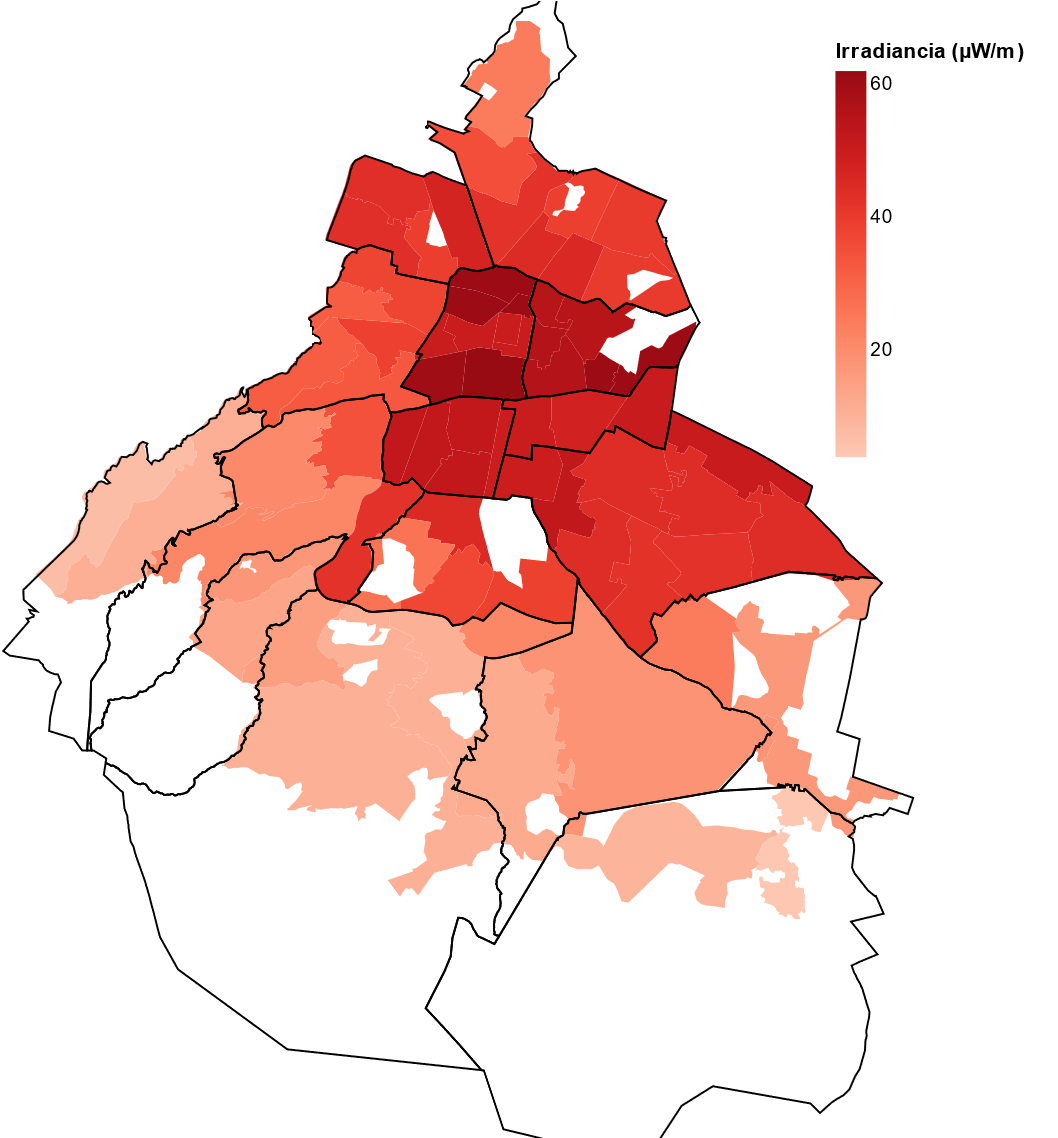
\includegraphics[width=1\textwidth]{MapaCLCDMX}
  \caption{Mapa CL-CDMX} 
  \label{MapaCLDMX}
\end{figure}

\newpage

Espacio para explicar el mapa y su buena reproducción de observaciones. irradiancia sobre una superficie horizntal
